\chapter{Análise de Distribuição e Normalidade}
\label{chap:analise_distribuicao_normalidade}

Nesta seção, investigamos a forma das distribuições das métricas de conectividade, tanto em seus valores "puros" quanto nas diferenças (\texttt{median\_diff}) entre as condições (Pós – Pré). Inicialmente, apresentamos as distribuições originais das métricas específicas \textbf{(PLI para EEG-EEG e CF-PLM para EEG-ECG)} que serão mantidas para análise. Em seguida, explicamos que, para testar o efeito da estimulação, calculamos a diferença entre os valores pós e pré (por exemplo, \emph{pós-sham} menos \emph{pré-sham}), e por fim discutimos a escolha dos testes estatísticos com base nessas distribuições.

\section{Distribuição das Métricas de Conectividade}

Antes de subtrair os valores pré dos pós, as métricas de conectividade foram extraídas diretamente dos sinais, refletindo as medidas originais sem a influência do efeito de estimulação. As figuras a seguir ilustram as distribuições "puras" para:

\begin{itemize}
    \item \textbf{PLI (EEG-EEG):} Avalia a sincronização de fase iso-frequencial entre canais cerebrais de EEG.
    \item \textbf{CF-PLM (EEG-ECG):} Mede o acoplamento \emph{cross-frequency} entre o EEG e o ciclo cardíaco obtido via ECG.
\end{itemize}

As faixas de frequência investigadas incluem: delta, theta, alpha, beta e gamma.

% -----------------------------------------------------------------------------  
% CF-PLM (EEG-ECG)  
% -----------------------------------------------------------------------------  
\begin{figure}[htb]
    \centering
    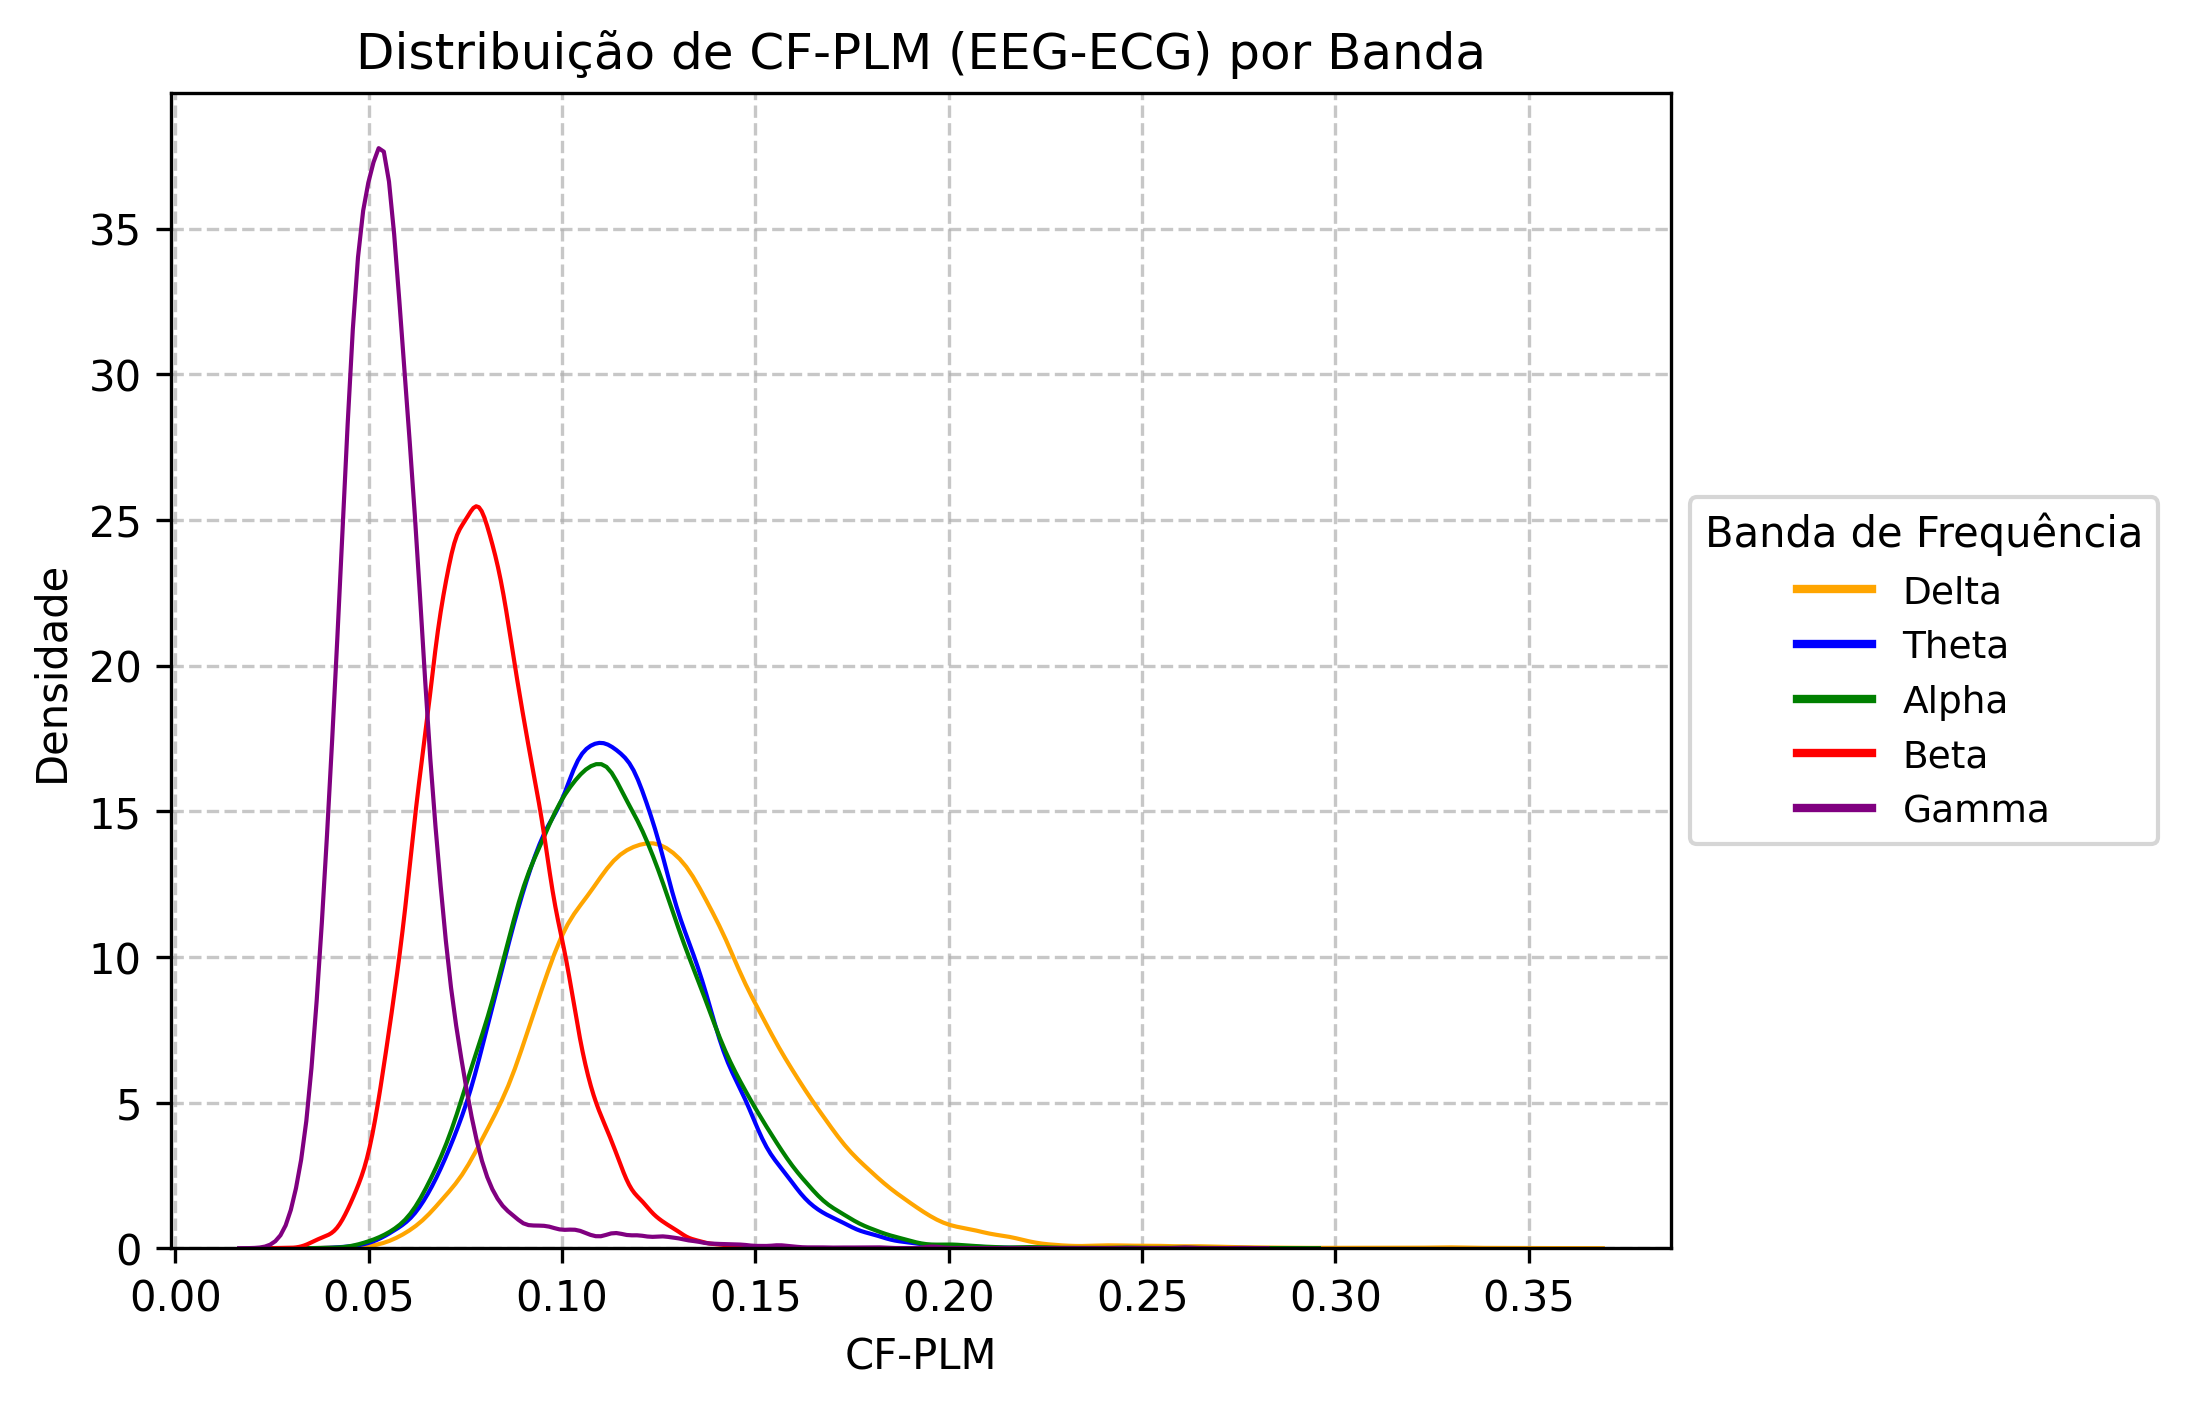
\includegraphics[width=0.7\textwidth]{figs/3_1_connectivity_metrics/Distribuição_de_CF-PLM_(EEG-ECG)_por_Banda.png}
    \caption{Distribuição de CF-PLM (EEG-ECG) por banda. Observa-se a concentração dos valores em faixas mais baixas (próximas de 0), com maior densidade para as bandas delta e theta.}
    \label{fig:cfplm_eeg_ecg}
\end{figure}

% -----------------------------------------------------------------------------  
% PLI (EEG-EEG)  
% -----------------------------------------------------------------------------  
\begin{figure}[htb]
    \centering
    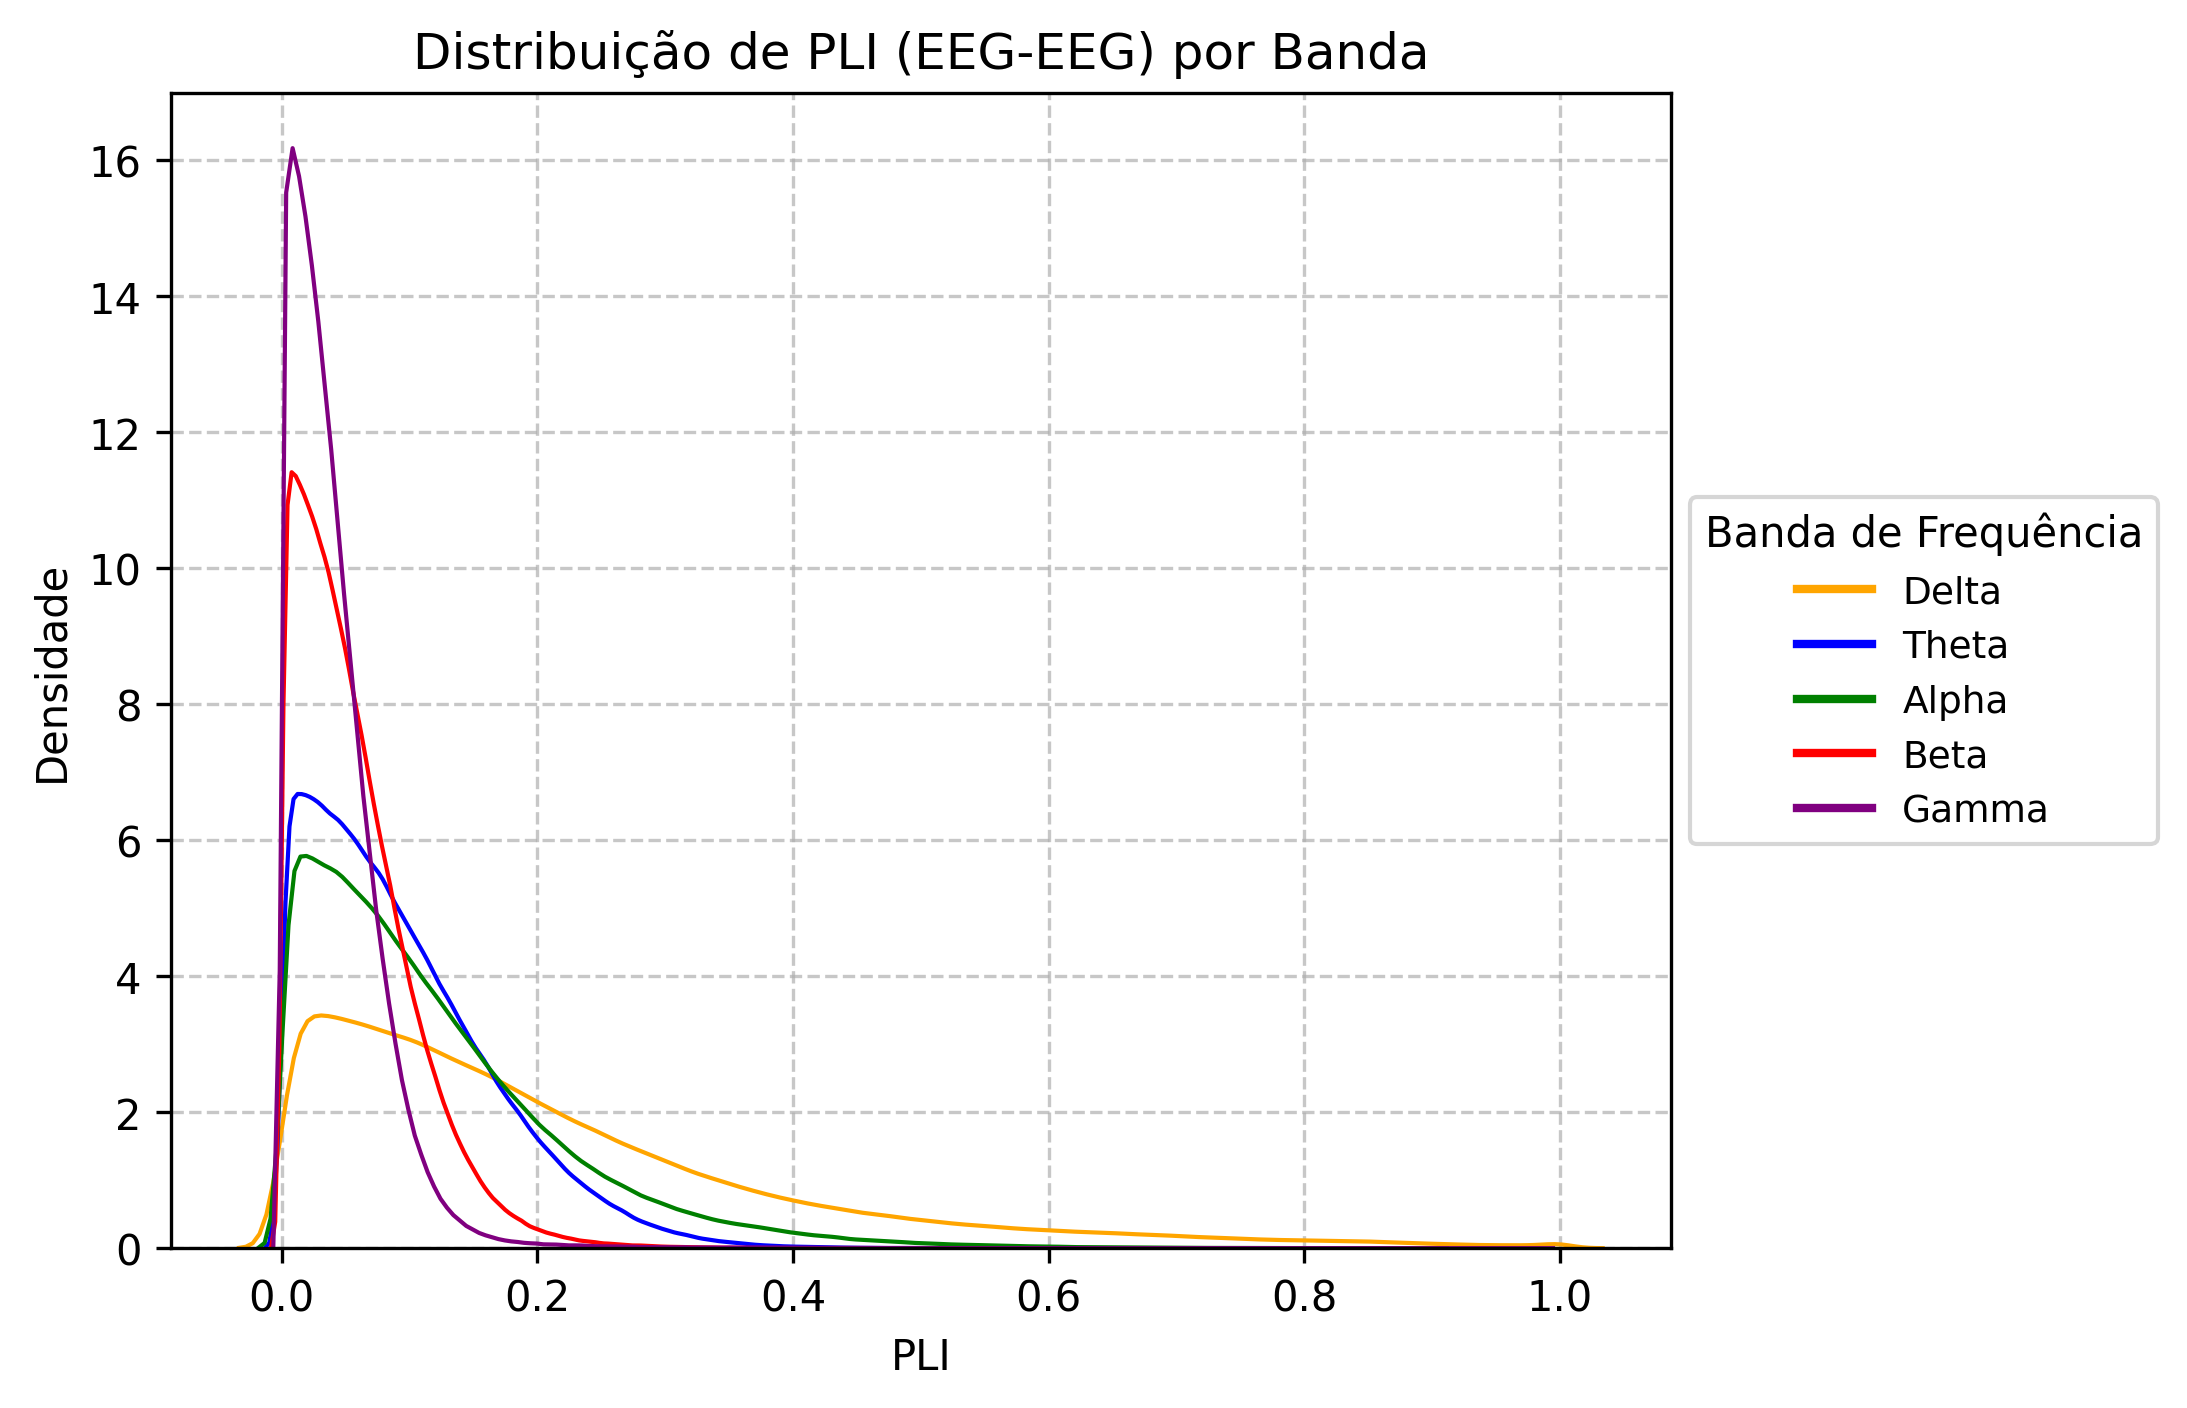
\includegraphics[width=0.7\textwidth]{figs/3_1_connectivity_metrics/Distribuição_de_PLI_(EEG-EEG)_por_Banda.png}
    \caption{Distribuição de PLI (EEG-EEG) por banda. Embora a maior parte dos valores se concentre em torno de zero, algumas bandas (alpha e gamma) apresentam caudas mais extensas, indicando pares de canais com defasagem de fase mais consistente.}
    \label{fig:pli_eeg_eeg}
\end{figure}

No geral, observamos que:
\begin{itemize}
    \item \textbf{EEG-EEG (PLI):} A distribuição pode se estender para valores elevados, sugerindo a presença de sincronizações robustas em algumas bandas.
    \item \textbf{EEG-ECG (CF-PLM):} Os valores geralmente se concentram próximos a zero, embora haja variações que indicam acoplamento \emph{cross-frequency} pontual.
\end{itemize}

Essas observações fornecem uma visão inicial do comportamento das métricas "puras" de conectividade, servindo de base para a comparação entre as condições (Pós e Pré), que será apresentada a seguir.

\section{Distribuição das Diferenças (\texttt{median\_diff})}

Para testar o efeito da estimulação (cathodic versus sham), comparamos os valores medidos após a intervenção (Pós) com os valores obtidos antes (Pré). Definimos a métrica:

\[
\texttt{median\_diff} = (\text{pós}) - (\text{pré}),
\]

o que visa isolar o efeito da intervenção, removendo variações comuns que estariam presentes independentemente da estimulação.

As distribuições das diferenças foram avaliadas por meio de histogramas com \emph{Kernel Density Estimation} (KDE) para as métricas utilizadas nesta análise (PLI para EEG-EEG e CF-PLM para EEG-ECG).

A seguir, ilustram-se exemplos desses histogramas:

% Exemplo: PLI (EEG-EEG) Diferença
\begin{figure}[htb]
    \centering
    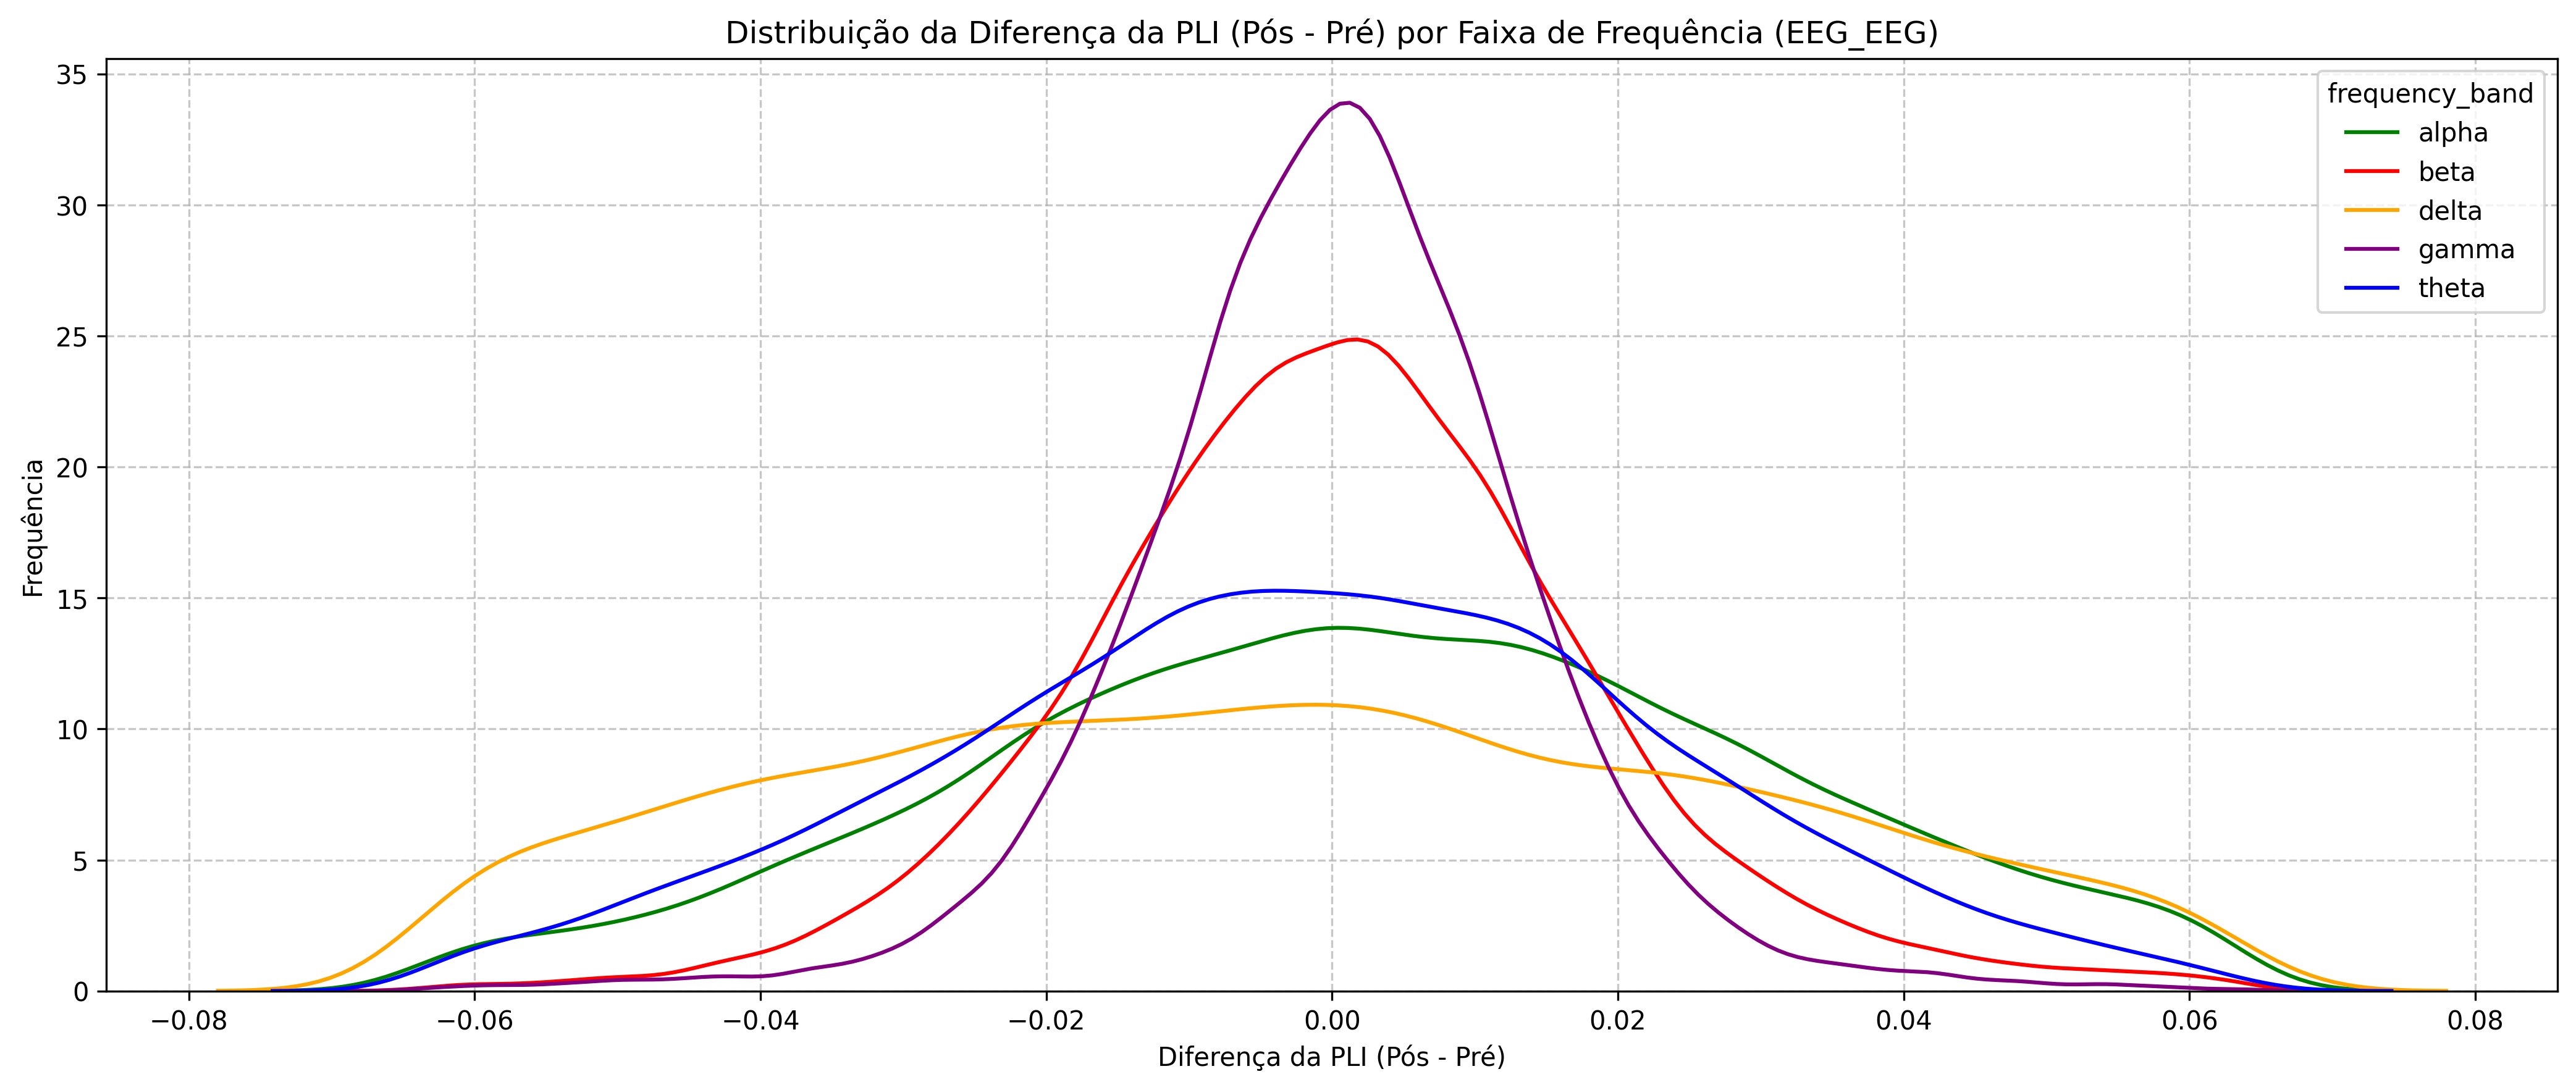
\includegraphics[width=0.8\textwidth]{figs/6_distribuicao_metricas_conectividade/Distribuição_da_Diferença_da_PLI_(Pós_-_Pré)_por_Faixa_de_Frequência_EEG_EEG.png}
    \caption{Distribuição da diferença da PLI (Pós -- Pré) em EEG-EEG, por faixa de frequência.}
    \label{fig:pli_freq_eeg_eeg}
\end{figure}

% Exemplo: CF-PLM (EEG-ECG) Diferença
\begin{figure}[htb]
    \centering
    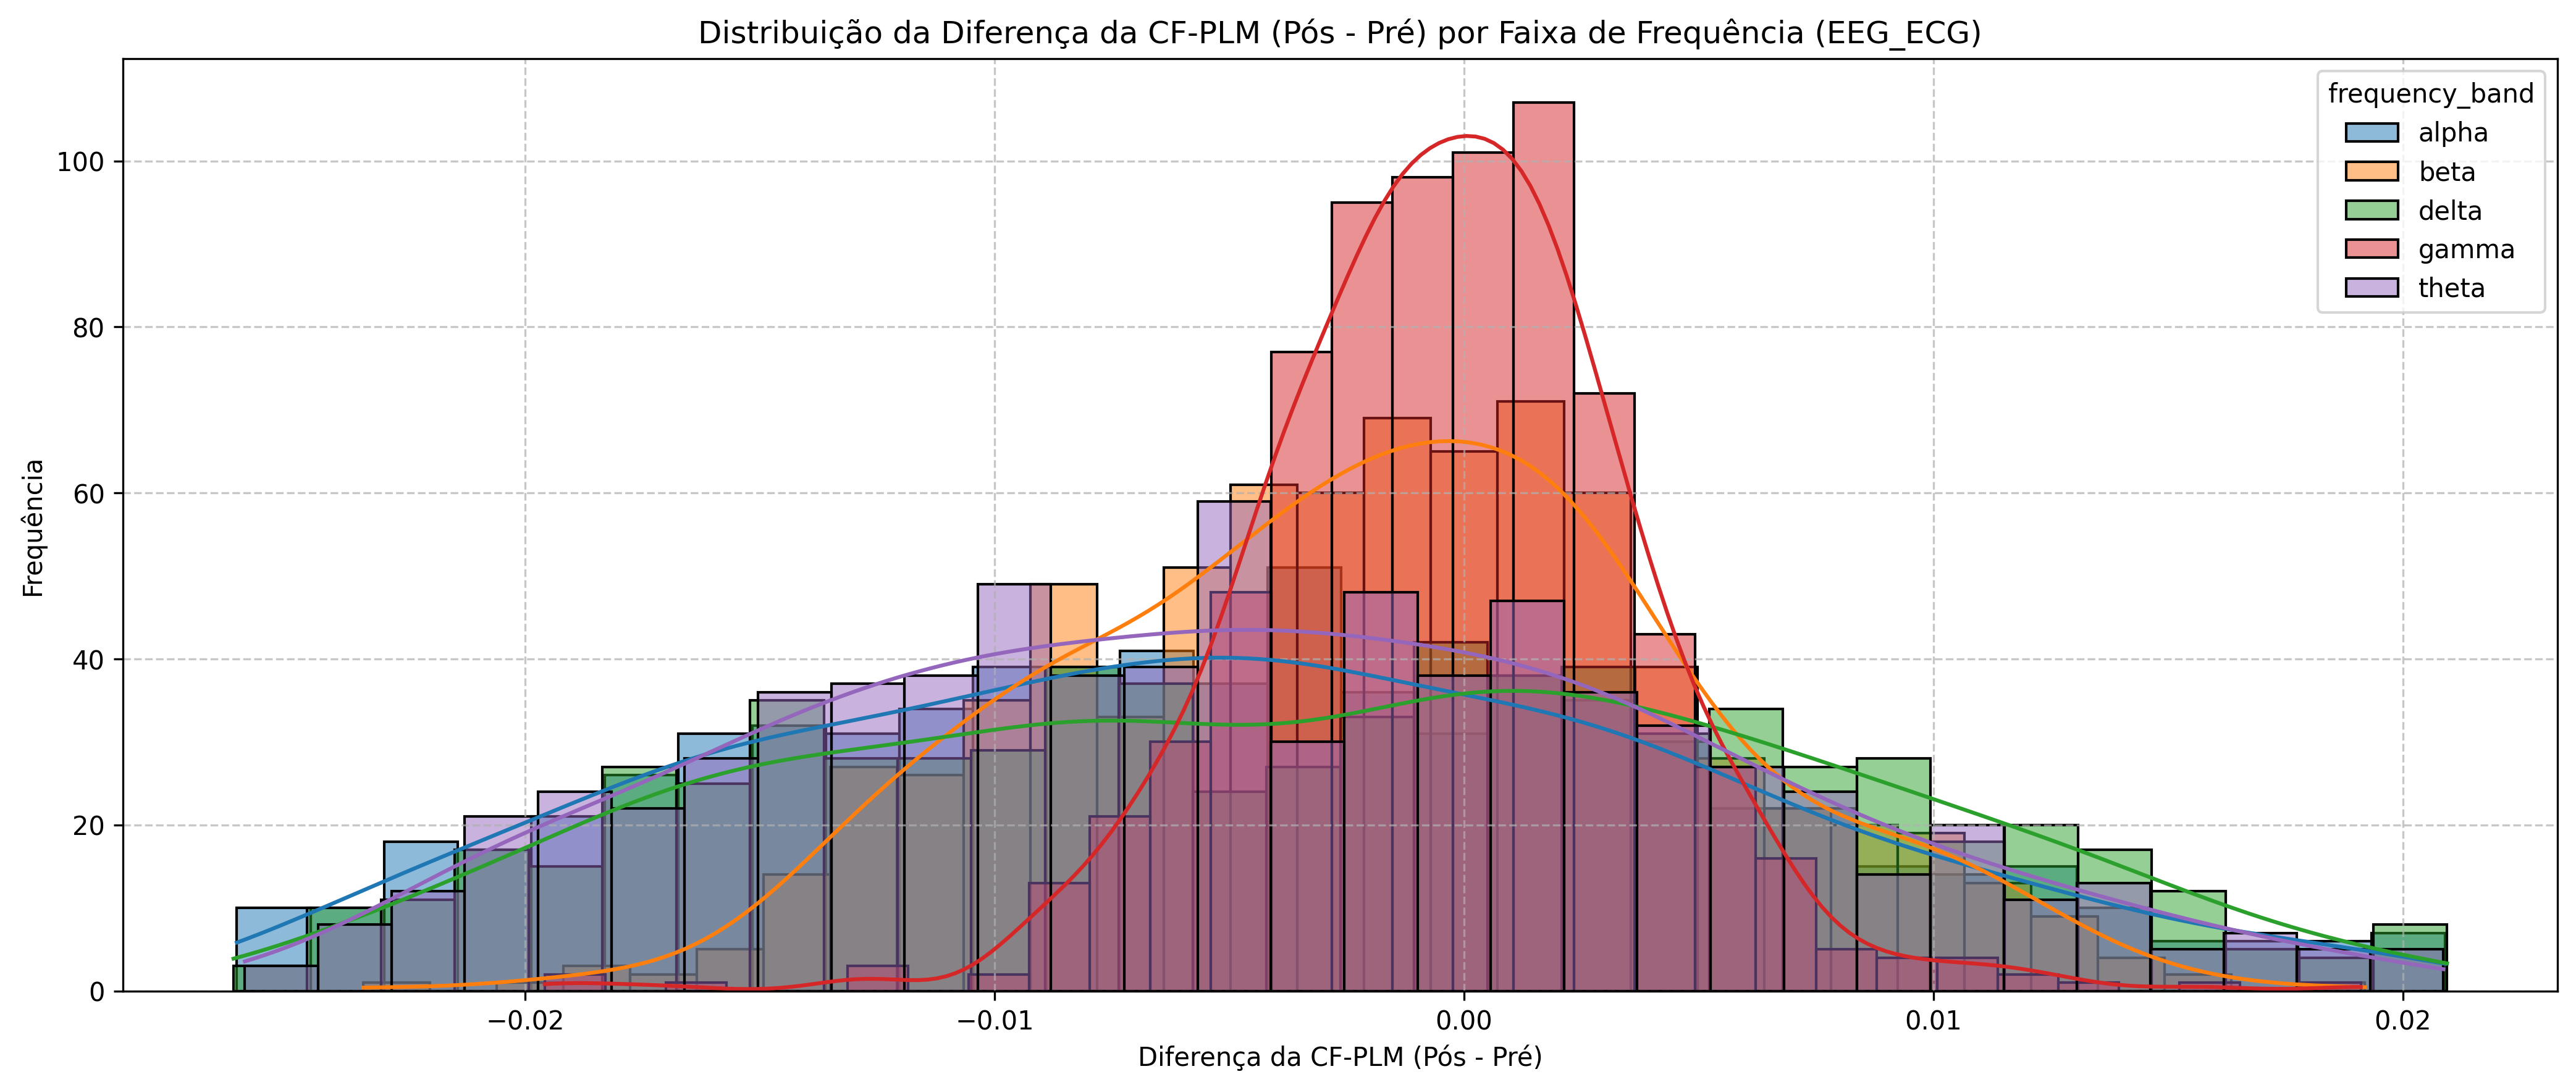
\includegraphics[width=0.8\textwidth]{figs/6_distribuicao_metricas_conectividade/Distribuição_da_Diferença_da_CF-PLM_(Pós_-_Pré)_por_Faixa_de_Frequência_EEG_ECG.png}
    \caption{Distribuição da diferença da CF-PLM (Pós -- Pré) em EEG-ECG, por faixa de frequência.}
    \label{fig:cf_plm_freq_eeg_ecg}
\end{figure}

Esses histogramas permitem visualizar como cada métrica (PLI ou CF-PLM) varia entre as condições Pós e Pré em diferentes faixas de frequência e fundamentam a escolha dos testes estatísticos, que serão discutidos no próximo capítulo.
\subsubsection{Exemplo Individual por Métrica e Banda}
Para ilustrar de forma mais específica o comportamento das distribuições em um caso individual, a Figura~\ref{fig:median_cf_plm_diff_ath4_alpha_eeg_ecg} exibe a distribuição da diferença da métrica \texttt{median\_cf\_plm\_diff} (Pós -- Pré) para o atleta 4, na banda \emph{alpha}, em pares EEG-ECG. De forma semelhante, a Figura~\ref{fig:median_pli_diff_ath4_alpha_eeg_eeg} apresenta a distribuição da diferença da métrica \texttt{median\_pli\_diff} para o mesmo atleta e banda, porém em pares EEG-EEG.

\begin{figure}[htb]
    \centering
    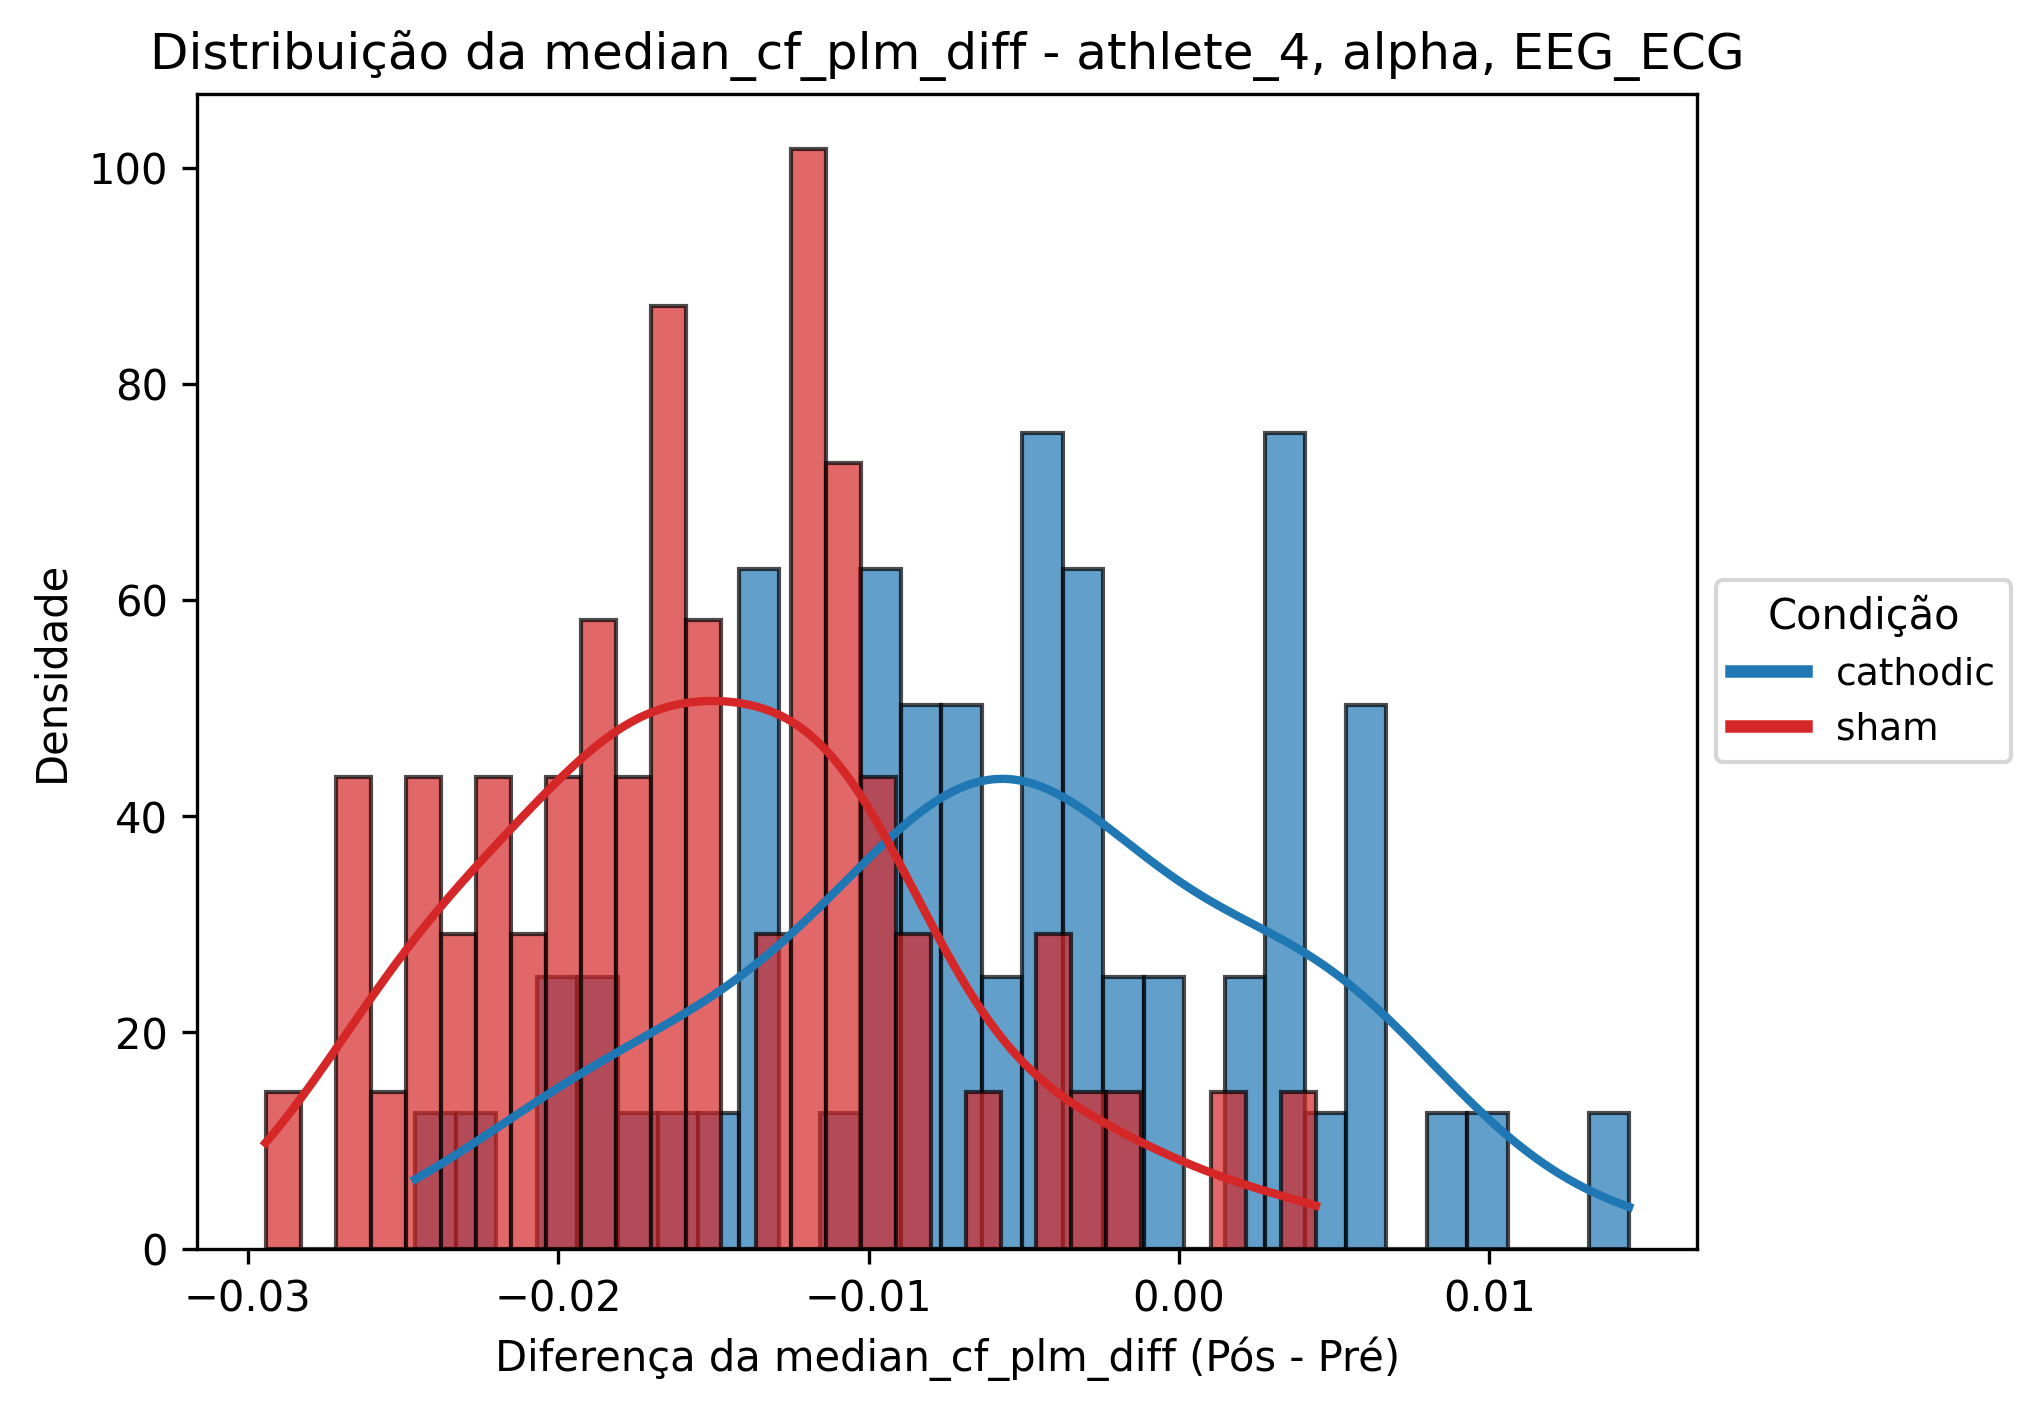
\includegraphics[width=0.8\textwidth]{figs/5_connectivity_metrics_individual_distribution/median_cf_plm_diff_athlete_4_alpha_EEG_ECG.png}
    \caption{Distribuição da \texttt{median\_cf\_plm\_diff} (Pós -- Pré) para o atleta 4, banda alpha, em pares EEG-ECG.}
    \label{fig:median_cf_plm_diff_ath4_alpha_eeg_ecg}
\end{figure}

\begin{figure}[htb]
    \centering
    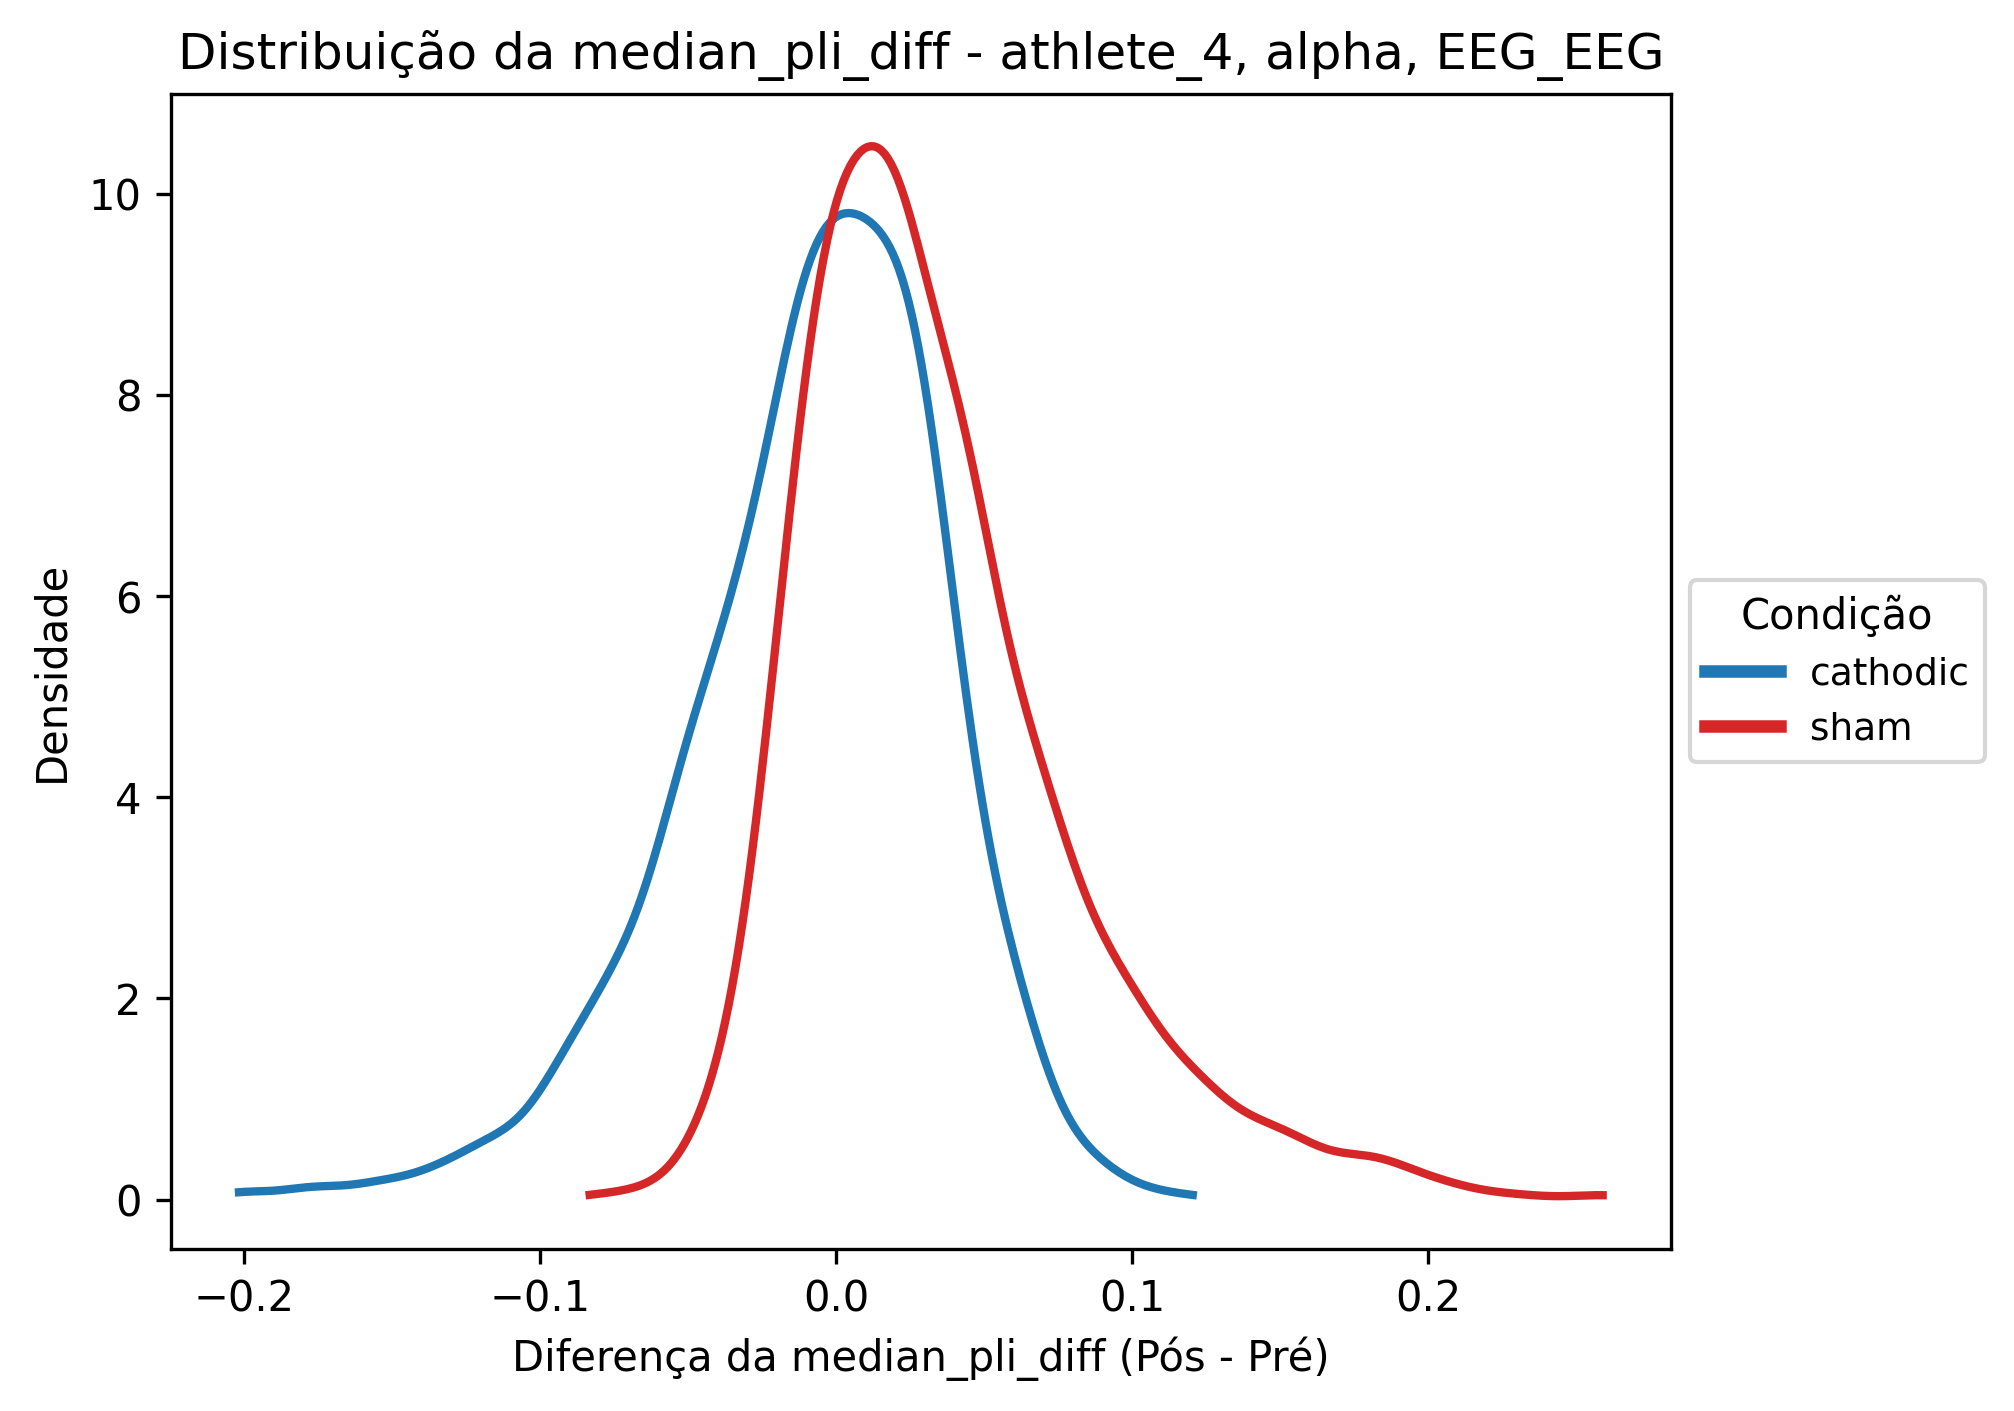
\includegraphics[width=0.8\textwidth]{figs/5_connectivity_metrics_individual_distribution/median_pli_diff_athlete_4_alpha_EEG_EEG.png}
    \caption{Distribuição da \texttt{median\_pli\_diff} (Pós -- Pré) para o atleta 4, banda alpha, em pares EEG-EEG.}
    \label{fig:median_pli_diff_ath4_alpha_eeg_eeg}
\end{figure}

Essas figuras exemplificam como as diferenças entre as condições \emph{cathodic} (azul) e \emph{sham} (vermelho) podem se sobrepor ou divergir. Em alguns casos, a curva KDE de uma condição desloca-se para a direita (indicando aumento da métrica após a estimulação) ou para a esquerda (indicando redução), enquanto em outros há significativa sobreposição, sugerindo pouca variação entre as condições. Esse tipo de análise individual é útil para verificar a variabilidade intra-sujeito e compreender se os efeitos observados são consistentes ou pontuais.

\section{Verificação de Normalidade e Escolha do Teste Estatístico}
Para definir se os testes estatísticos a serem empregados serão paramétricos ou não-paramétricos, é necessário verificar a normalidade das distribuições de interesse. Nesse contexto, testes como Shapiro-Wilk e Kolmogorov-Smirnov podem ser aplicados para cada grupo de canais e faixa de frequência, tanto para as métricas de PLI quanto para as de CF-PLM.

\paragraph{Considerações:}
\begin{itemize}
    \item \textbf{Tamanho amostral:} Dada a grande quantidade de observações após agregação, mesmo pequenas diferenças em relação à normalidade podem levar à rejeição da hipótese nula.
    \item \textbf{Forma das distribuições:} Visualmente, muitas distribuições parecem simétricas e unimodais, mas pequenas assimetrias ou caudas alongadas podem requerer cautela ao adotar testes paramétricos.
    \item \textbf{Interpretação:} Se a maioria das distribuições apresentar p-valores inferiores a 0.05 nos testes de normalidade, a análise inferencial subsequente deve se apoiar em testes não-paramétricos (por exemplo, Wilcoxon signed-rank ou Mann-Whitney).
\end{itemize}

\paragraph{Próximos Passos:}
\begin{itemize}
    \item Realizar os testes de normalidade (Shapiro-Wilk e/ou Kolmogorov-Smirnov) para cada combinação relevante de faixa de frequência e grupo de canais.
    \item Avaliar medidas de assimetria (skewness) e curtose (kurtosis) para confirmar a adequação de testes paramétricos ou justificar o uso de métodos não-paramétricos.
\end{itemize}

Com base nessa análise preliminar, será possível conduzir as etapas subsequentes de inferência estatística, levando em conta as particularidades de cada métrica (PLI e CF-PLM) e garantindo uma avaliação robusta das diferenças entre condições.

\section{Testes de Normalidade e Decisão sobre o Tipo de Teste Estatístico}
A escolha entre testes paramétricos e não-paramétricos depende fundamentalmente da distribuição dos dados. Para as métricas de conectividade (\texttt{median\_pli\_diff} e \texttt{median\_cf\_plm\_diff}) agrupadas nos grupos \texttt{EEG\_EEG} e \texttt{EEG\_ECG}, aplicamos uma série de testes de normalidade, a saber: Shapiro-Wilk, Kolmogorov-Smirnov, Anderson-Darling, D'Agostino's K-squared, Jarque-Bera e Lilliefors. Além disso, para atenuar o efeito de valores extremos, os testes foram realizados tanto com os dados originais quanto após a remoção de outliers utilizando o método do Interquartile Range (IQR).

\paragraph{Motivações e Procedimentos:}
\begin{itemize}
    \item \textbf{Objetivo:} Verificar se as distribuições das diferenças (Pós -- Pré) seguem uma forma aproximadamente gaussiana, o que permitiria o uso de testes paramétricos.
    \item \textbf{Procedimento:} 
    \begin{itemize}
        \item Os dados foram agrupados por \texttt{channel\_group} (EEG\_EEG e EEG\_ECG) e por métrica.
        \item Os testes de normalidade foram aplicados com e sem outliers, permitindo avaliar o efeito destes na distribuição.
    \end{itemize}
\end{itemize}

\paragraph{Principais Resultados:}
\begin{itemize}
    \item \textbf{Grupo EEG\_EEG (PLI):}
    \begin{itemize}
        \item Para \texttt{median\_pli\_diff}, todos os testes (Shapiro-Wilk, Kolmogorov-Smirnov, Anderson-Darling, D'Agostino, Jarque-Bera e Lilliefors) indicaram desvios significativos da normalidade (p-valores muito baixos), mesmo após a remoção de outliers (10,66\% dos dados).
    \end{itemize}
    \item \textbf{Grupo EEG\_ECG (CF-PLM):}
    \begin{itemize}
        \item Para \texttt{median\_cf\_plm\_diff}, mesmo após a remoção de outliers (10,65\% dos dados), os testes continuaram a rejeitar a normalidade, com p-valores próximos de zero na maioria dos casos.
    \end{itemize}
\end{itemize}

\paragraph{Interpretação e Decisão Metodológica:}
Os resultados dos testes de normalidade indicam que, em sua maioria, as distribuições das diferenças das métricas de conectividade não se comportam de forma normal, mesmo após a remoção de outliers. Essa violação dos pressupostos de normalidade sugere que a aplicação de testes paramétricos poderia levar a inferências incorretas. Portanto, optou-se por utilizar testes não-paramétricos para as análises estatísticas subsequentes, garantindo robustez e validade às conclusões sem a necessidade de assumir normalidade dos dados.
